\begin{align*}
    \polynomialP{1}{N}{0} &= 0 \\
    \polynomialP{1}{N}{1} &= 6N - 5 \\
    \polynomialP{1}{N}{2} &= 18N - 28 \\
    \polynomialP{1}{N}{3} &= 36N - 81 \\
    \polynomialP{1}{N}{4} &= 60N - 176 \\
    \polynomialP{1}{N}{5} &= 90N - 325 \\
    \polynomialP{1}{N}{6} &= 126N - 540 \\
    \polynomialP{1}{N}{7} &= 168N - 833 \\
    \polynomialP{1}{N}{8} &= 216N - 1216 \\
    \polynomialP{1}{N}{9} &= 270N - 1701 \\
    \polynomialP{1}{N}{10} &= 330N - 2300 \\
    \polynomialP{1}{N}{11} &= 396N - 3025 \\
    \polynomialP{1}{N}{12} &= 468N - 3888 \\
    \polynomialP{1}{N}{13} &= 546N - 4901 \\
    \polynomialP{1}{N}{14} &= 630N - 6076 \\
    \polynomialP{1}{N}{15} &= 720N - 7425 \\
    \polynomialP{1}{N}{16} &= 816N - 8960 \\
    \polynomialP{1}{N}{17} &= 918N - 10693 \\
    \polynomialP{1}{N}{18} &= 1026N - 12636 \\
    \polynomialP{1}{N}{19} &= 1140N - 14801 \\
    \polynomialP{1}{N}{20} &= 1260N - 17200
\end{align*}
\begin{figure}[H]
    \centering
    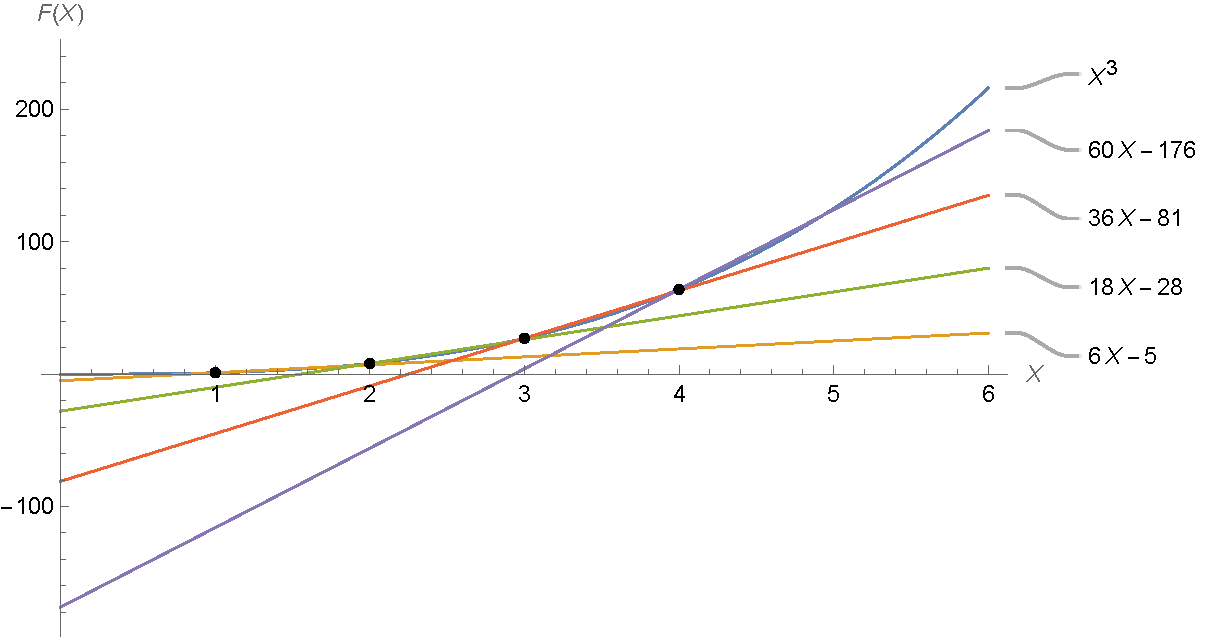
\includegraphics[width=1\textwidth]{sections/images/01_cubes_with_p_1_n_k}
    ~\caption{Polynomials P(1, n, k)}\label{fig:figure}
\end{figure}
